% Options for packages loaded elsewhere
\PassOptionsToPackage{unicode}{hyperref}
\PassOptionsToPackage{hyphens}{url}
%
\documentclass[
]{article}
\usepackage{lmodern}
\usepackage{amssymb,amsmath}
\usepackage{ifxetex,ifluatex}
\ifnum 0\ifxetex 1\fi\ifluatex 1\fi=0 % if pdftex
  \usepackage[T1]{fontenc}
  \usepackage[utf8]{inputenc}
  \usepackage{textcomp} % provide euro and other symbols
\else % if luatex or xetex
  \usepackage{unicode-math}
  \defaultfontfeatures{Scale=MatchLowercase}
  \defaultfontfeatures[\rmfamily]{Ligatures=TeX,Scale=1}
\fi
% Use upquote if available, for straight quotes in verbatim environments
\IfFileExists{upquote.sty}{\usepackage{upquote}}{}
\IfFileExists{microtype.sty}{% use microtype if available
  \usepackage[]{microtype}
  \UseMicrotypeSet[protrusion]{basicmath} % disable protrusion for tt fonts
}{}
\makeatletter
\@ifundefined{KOMAClassName}{% if non-KOMA class
  \IfFileExists{parskip.sty}{%
    \usepackage{parskip}
  }{% else
    \setlength{\parindent}{0pt}
    \setlength{\parskip}{6pt plus 2pt minus 1pt}}
}{% if KOMA class
  \KOMAoptions{parskip=half}}
\makeatother
\usepackage{xcolor}
\IfFileExists{xurl.sty}{\usepackage{xurl}}{} % add URL line breaks if available
\IfFileExists{bookmark.sty}{\usepackage{bookmark}}{\usepackage{hyperref}}
\hypersetup{
  pdftitle={mikropml: User-Friendly R Package for Supervised Machine Learning Pipelines},
  pdfauthor={Begüm D. Topçuoğlu, Zena Lapp, Kelly L. Sovacool, Evan Snitkin, Jenna Wiens, Patrick D. Schloss},
  hidelinks,
  pdfcreator={LaTeX via pandoc}}
\urlstyle{same} % disable monospaced font for URLs
\usepackage[margin=1in]{geometry}
\usepackage{graphicx,grffile}
\makeatletter
\def\maxwidth{\ifdim\Gin@nat@width>\linewidth\linewidth\else\Gin@nat@width\fi}
\def\maxheight{\ifdim\Gin@nat@height>\textheight\textheight\else\Gin@nat@height\fi}
\makeatother
% Scale images if necessary, so that they will not overflow the page
% margins by default, and it is still possible to overwrite the defaults
% using explicit options in \includegraphics[width, height, ...]{}
\setkeys{Gin}{width=\maxwidth,height=\maxheight,keepaspectratio}
% Set default figure placement to htbp
\makeatletter
\def\fps@figure{htbp}
\makeatother
\setlength{\emergencystretch}{3em} % prevent overfull lines
\providecommand{\tightlist}{%
  \setlength{\itemsep}{0pt}\setlength{\parskip}{0pt}}
\setcounter{secnumdepth}{-\maxdimen} % remove section numbering

\title{mikropml: User-Friendly R Package for Supervised Machine Learning
Pipelines}
\author{Begüm D. Topçuoğlu, Zena Lapp, Kelly L. Sovacool, Evan Snitkin, Jenna
Wiens, Patrick D. Schloss}
\date{2021-01-22}

\begin{document}
\maketitle

\hypertarget{summary}{%
\section{Summary}\label{summary}}

Machine learning (ML) for classification and prediction based on a set
of features is used to make decisions in healthcare, economics, criminal
justice and more. However, implementing an ML pipeline including
preprocessing, model selection, and evaluation can be time-consuming,
confusing, and difficult. Here, we present
\href{http://www.schlosslab.org/mikropml/}{\texttt{mikropml}} (prononced
``meek-ROPE em el''), an easy-to-use R package that implements ML
pipelines using regression, support vector machines, decision trees,
random forest, or gradient-boosted trees. The package is available on
\href{https://github.com/SchlossLab/mikropml/}{GitHub},
\href{https://cran.r-project.org/package=mikropml}{CRAN}, and
\href{https://anaconda.org/conda-forge/r-mikropml}{conda}.

\hypertarget{statement-of-need}{%
\section{Statement of need}\label{statement-of-need}}

Most applications of machine learning (ML) require reproducible steps
for data pre-processing, cross-validation, testing, model evaluation,
and often interpretation of why the model makes particular predictions.
Performing these steps is important, as failure to implement them can
result in incorrect and misleading results (Teschendorff 2019; Wiens et
al. 2019).

Supervised ML is widely used to recognize patterns in large datasets and
to make predictions about outcomes of interest. Several packages
including \texttt{caret} (Kuhn 2008) and \texttt{tidymodels} (Kuhn,
Wickham, and RStudio 2020) in R, \texttt{scikitlearn} (Pedregosa et al.
2011) in Python, and the H2O \texttt{autoML} platform (H2O.ai 2020)
allow scientists to train ML models with a variety of algorithms. While
these packages provide the tools necessary for each ML step, they do not
implement a complete ML pipeline according to good practices in the
literature. This makes it difficult for practitioners new to ML to
easily begin to perform ML analyses.

To enable a broader range of researchers to apply ML to their problem
domains, we created
\href{https://github.com/SchlossLab/mikropml/}{\texttt{mikropml}}, an
easy-to-use R package (R Core Team 2020) that implements the ML pipeline
created by Topçuoğlu \emph{et al.} (Topçuoğlu et al. 2020) in a single
function that returns a trained model, model performance metrics and
feature importance. \texttt{mikropml} leverages the \texttt{caret}
package to support several ML algorithms: linear regression, logistic
regression, support vector machines with a radial basis kernel, decision
trees, random forest, and gradient boosted trees. It incorporates good
practices in ML training, testing, and model evaluation (Topçuoğlu et
al. 2020; Teschendorff 2019). Furthermore, it provides data
preprocessing steps based on the FIDDLE (FlexIble Data-Driven pipeLinE)
framework outlined in Tang \emph{et al.} (Tang et al. 2020) and
post-training permutation importance steps to estimate the importance of
each feature in the models trained (Breiman 2001; Fisher, Rudin, and
Dominici 2018).

\texttt{mikropml} can be used as a starting point in the application of
ML to datasets from many different fields. It has already been applied
to microbiome data to categorize patients with colorectal cancer
(Topçuoğlu et al. 2020), to identify differences in genomic and clinical
features associated with bacterial infections (Lapp et al. 2020), and to
predict gender-based biases in academic publishing (Hagan et al. 2020).

\hypertarget{mikropml-package}{%
\section{mikropml package}\label{mikropml-package}}

The \texttt{mikropml} package includes functionality to preprocess the
data, train ML models, evaluate model performance, and quantify feature
importance (Figure 1). We also provide
\href{http://www.schlosslab.org/mikropml/articles/index.html}{vignettes}
and an
\href{https://github.com/SchlossLab/mikropml-snakemake-workflow}{example
Snakemake workflow} (Köster and Rahmann 2012) to showcase how to run an
ideal ML pipeline with multiple different train/test data splits. The
results can be visualized using helper functions that use
\texttt{ggplot2} (Wickham 2016).

While mikropml allows users to get started quickly and facilitates
reproducibility, it is not a replacement for understanding the ML
workflow which is still necessary when interpreting results (Pollard et
al. 2019). To facilitate understanding and enable one to tailor the code
to their application, we have heavily commented the code and have
provided supporting documentation which can be read
\href{http://www.schlosslab.org/mikropml/}{online}.

\hypertarget{preprocessing-data}{%
\subsection{Preprocessing data}\label{preprocessing-data}}

We provide the function \texttt{preprocess\_data()} to preprocess
features using several different functions from the \texttt{caret}
package. \texttt{preprocess\_data()} takes continuous and categorical
data, re-factors categorical data into binary features, and provides
options to normalize continuous data, remove features with near-zero
variance, and keep only one instance of perfectly correlated features.
We set the default options based on those implemented in FIDDLE (Tang et
al. 2020). More details on how to use \texttt{preprocess\_data()} can be
found in the accompanying
\href{http://www.schlosslab.org/mikropml/articles/preprocess.html}{vignette}.

\hypertarget{running-ml}{%
\subsection{Running ML}\label{running-ml}}

The main function in mikropml, \texttt{run\_ml()}, minimally takes in
the model choice and a data frame with an outcome column and feature
columns. For model choice, \texttt{mikropml} currently supports logistic
and linear regression (\texttt{glmnet}: Friedman, Hastie, and Tibshirani
2010), support vector machines with a radial basis kernel
(\texttt{kernlab}: Karatzoglou et al. 2004), decision trees
(\texttt{rpart}: Therneau et al. 2019), random forest
(\texttt{randomForest}: Liaw and Wiener 2002), and gradient-boosted
trees (\texttt{xgboost}: Chen et al. 2020). \texttt{run\_ml()} randomly
splits the data into train and test sets while maintaining the
distribution of the outcomes found in the full dataset. It also provides
the option to split the data into train and test sets based on
categorical variables (e.g.~batch, geographic location, etc.).
\texttt{mikropml} uses the \texttt{caret} package (Kuhn 2008) to train
and evaluate the models, and optionally quantifies feature importance.
The output includes the best model built based on tuning hyperparameters
in an internal and repeated cross-validation step, model evaluation
metrics, and optional feature importances. Feature importances are
calculated using a permutation test, which breaks the relationship
between the feature and the true outcome in the test data, and measures
the change in model performance. This provides an intuitive metric of
how individual features influence model performance and is comparable
across model types, which is particularly useful for model
interpretation (Topçuoğlu et al. 2020). Our
\href{http://www.schlosslab.org/mikropml/articles/introduction.html}{introductory
vignette} contains a comprehensive tutorial on how to use
\texttt{run\_ml()}.

\begin{figure}
\centering
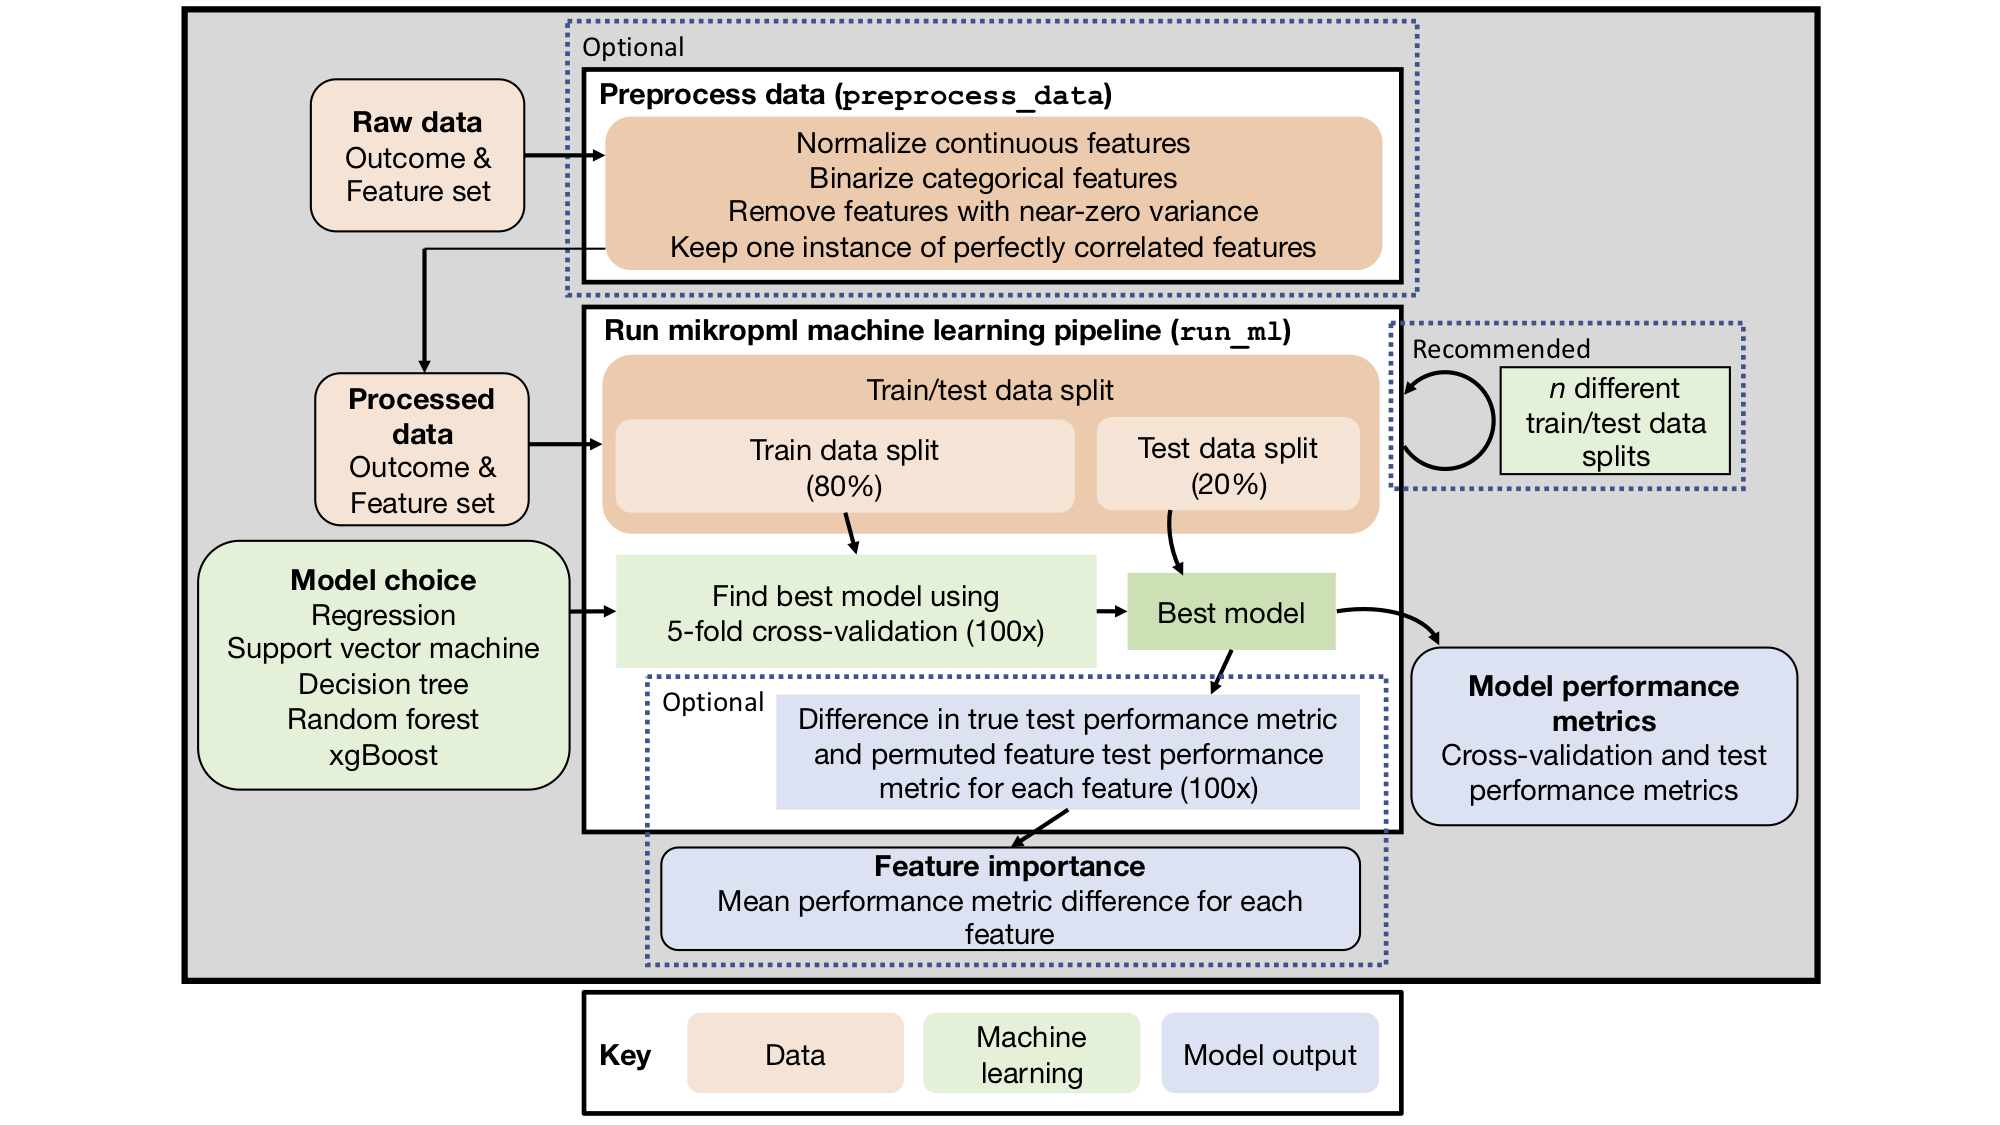
\includegraphics[width=1\textwidth,height=\textheight]{mikRopML-pipeline.png}
\caption{mikropml pipeline}
\end{figure}

\hypertarget{ideal-workflow-for-running-mikropml-with-many-different-traintest-splits}{%
\subsection{Ideal workflow for running mikropml with many different
train/test
splits}\label{ideal-workflow-for-running-mikropml-with-many-different-traintest-splits}}

To investigate the variation in model performance depending on the train
and test set used (Topçuoğlu et al. 2020; Lapp et al. 2020), we provide
examples of how to \texttt{run\_ml()} many times with different
train/test splits and how to get summary information about model
performance on
\href{http://www.schlosslab.org/mikropml/articles/parallel.html}{a local
computer} or on a high-performance computing cluster using a
\href{https://github.com/SchlossLab/mikropml-snakemake-workflow}{Snakemake
workflow}.

\hypertarget{tuning-visualization}{%
\subsection{Tuning \& visualization}\label{tuning-visualization}}

One particularly important aspect of ML is hyperparameter tuning. We
provide a reasonable range of default hyperparameters for each model
type. However practitioners should explore whether that range is
appropriate for their data, or if they should customize the
hyperparameter range. Therefore, we provide a function
\texttt{plot\_hp\_performance()} to plot the cross-validation
performance metric of a single model or models built using different
train/test splits. This helps evaluate if the hyperparameter range is
being searched exhaustively and allows the user to pick the ideal set.
We also provide summary plots of test performance metrics for the many
train/test splits with different models using
\texttt{plot\_model\_performance()}. Examples are described in the
accompanying
\href{http://www.schlosslab.org/mikropml/articles/tuning.html}{vignette
on hyperparameter tuning}.

\hypertarget{dependencies}{%
\subsection{Dependencies}\label{dependencies}}

mikropml is written in R (R Core Team 2020) and depends on several
packages: \texttt{dplyr} (Wickham et al. 2020), \texttt{rlang} (Henry,
Wickham, and RStudio 2020) and \texttt{caret} (Kuhn 2008). The ML
algorithms supported by \texttt{mikropml} require: \texttt{glmnet}
(Friedman, Hastie, and Tibshirani 2010), \texttt{e1071} (Meyer et al.
2020), and \texttt{MLmetrics} (Yan 2016) for logistic regression,
\texttt{rpart2} (Therneau et al. 2019) for decision trees,
\texttt{randomForest} (Liaw and Wiener 2002) for random forest,
\texttt{xgboost} (Chen et al. 2020) for xgboost, and \texttt{kernlab}
(Karatzoglou et al. 2004) for support vector machines. We also allow for
parallelization of cross-validation and other steps using the
\texttt{foreach}, \texttt{doFuture}, \texttt{future.apply}, and
\texttt{future} packages (Bengtsson and Team 2020). Finally, we use
\texttt{ggplot2} for plotting (Wickham 2016).

\hypertarget{acknowledgments}{%
\section{Acknowledgments}\label{acknowledgments}}

We thank members of the Schloss Lab who participated in code clubs
related to the initial development of the pipeline, made documentation
improvements, and provided general feedback.

\hypertarget{funding}{%
\section{Funding}\label{funding}}

Salary support for PDS came from NIH grant 1R01CA215574. KLS received
support from the NIH Training Program in Bioinformatics (T32 GM070449).
ZL received support from the National Science Foundation Graduate
Research Fellowship Program under Grant No.~DGE 1256260. Any opinions,
findings, and conclusions or recommendations expressed in this material
are those of the authors and do not necessarily reflect the views of the
National Science Foundation.

\hypertarget{author-contributions}{%
\section{Author contributions}\label{author-contributions}}

BDT, ZL, and KLS contributed equally. Author order among the co-first
authors was determined by time since joining the project.

BDT, ZL, and KLS conceptualized the study and wrote the code. KLS
structured the code in R package form. BDT, ZL, JW, and PDS developed
methodology. PDS, ES, and JW supervised the project. BDT, ZL, and KLS
wrote the original draft. All authors reviewed and edited the
manuscript.

\hypertarget{conflicts-of-interest}{%
\section{Conflicts of interest}\label{conflicts-of-interest}}

None.

\hypertarget{references}{%
\section*{References}\label{references}}
\addcontentsline{toc}{section}{References}

\hypertarget{refs}{}
\leavevmode\hypertarget{ref-bengtsson_futureapply_2020}{}%
Bengtsson, Henrik, and R Core Team. 2020. ``Future.Apply: Apply Function
to Elements in Parallel Using Futures,'' July.

\leavevmode\hypertarget{ref-breiman_random_2001}{}%
Breiman, Leo. 2001. ``Random Forests.'' \emph{Machine Learning} 45 (1):
5--32. \url{https://doi.org/10.1023/A:1010933404324}.

\leavevmode\hypertarget{ref-chen_xgboost_2020}{}%
Chen, Tianqi, Tong He, Michael Benesty, Vadim Khotilovich, Yuan Tang,
Hyunsu Cho, Kailong Chen, et al. 2020. ``Xgboost: Extreme Gradient
Boosting,'' June.

\leavevmode\hypertarget{ref-fisher_all_2018}{}%
Fisher, Aaron, Cynthia Rudin, and Francesca Dominici. 2018. ``All Models
Are Wrong, but Many Are Useful: Learning a Variable's Importance by
Studying an Entire Class of Prediction Models Simultaneously.''

\leavevmode\hypertarget{ref-friedman_regularization_2010}{}%
Friedman, Jerome H., Trevor Hastie, and Rob Tibshirani. 2010.
``Regularization Paths for Generalized Linear Models via Coordinate
Descent.'' \emph{Journal of Statistical Software} 33 (1): 1--22.
\url{https://doi.org/10.18637/jss.v033.i01}.

\leavevmode\hypertarget{ref-h2o_platform}{}%
H2O.ai. 2020. \emph{H2O: Scalable Machine Learning Platform}. Manual.

\leavevmode\hypertarget{ref-hagan_women_2020}{}%
Hagan, Ada K., Begüm D. Topçuoğlu, Mia E. Gregory, Hazel A. Barton, and
Patrick D. Schloss. 2020. ``Women Are Underrepresented and Receive
Differential Outcomes at ASM Journals: A Six-Year Retrospective
Analysis.'' \emph{mBio} 11 (6).
\url{https://doi.org/10.1128/mBio.01680-20}.

\leavevmode\hypertarget{ref-henry_rlang_2020}{}%
Henry, Lionel, Hadley Wickham, and RStudio. 2020. ``Rlang: Functions for
Base Types and Core R and 'Tidyverse' Features,'' July.

\leavevmode\hypertarget{ref-karatzoglou_kernlab_2004}{}%
Karatzoglou, Alexandros, Alexandros Smola, Kurt Hornik, and Achim
Zeileis. 2004. ``Kernlab - an S4 Package for Kernel Methods in R.''
\emph{Journal of Statistical Software} 11 (1): 1--20.
\url{https://doi.org/10.18637/jss.v011.i09}.

\leavevmode\hypertarget{ref-koster_snakemakescalable_2012}{}%
Köster, Johannes, and Sven Rahmann. 2012. ``Snakemakea Scalable
Bioinformatics Workflow Engine.'' \emph{Bioinformatics} 28 (19):
2520--2. \url{https://doi.org/10.1093/bioinformatics/bts480}.

\leavevmode\hypertarget{ref-kuhn_building_2008}{}%
Kuhn, Max. 2008. ``Building Predictive Models in R Using the Caret
Package.'' \emph{Journal of Statistical Software} 28 (1): 1--26.
\url{https://doi.org/10.18637/jss.v028.i05}.

\leavevmode\hypertarget{ref-kuhn_tidymodels_2020}{}%
Kuhn, Max, Hadley Wickham, and RStudio. 2020. ``Tidymodels: Easily
Install and Load the 'Tidymodels' Packages,'' July.

\leavevmode\hypertarget{ref-lapp_machine_2020}{}%
Lapp, Zena, Jennifer Han, Jenna Wiens, Ellie JC Goldstein, Ebbing
Lautenbach, and Evan Snitkin. 2020. ``Machine Learning Models to
Identify Patient and Microbial Genetic Factors Associated with
Carbapenem-Resistant Klebsiella Pneumoniae Infection.'' \emph{medRxiv},
July, 2020.07.06.20147306.
\url{https://doi.org/10.1101/2020.07.06.20147306}.

\leavevmode\hypertarget{ref-liaw_classication_2002}{}%
Liaw, Andy, and Matthew Wiener. 2002. ``Classification and Regression by
randomForest'' 2: 5.

\leavevmode\hypertarget{ref-meyer_e1071_2020}{}%
Meyer, David, Evgenia Dimitriadou, Kurt Hornik, Andreas Weingessel,
Friedrich Leisch, Chih-Chung Chang (libsvm C++-code), and Chih-Chen Lin
(libsvm C++-code). 2020. ``E1071: Misc Functions of the Department of
Statistics, Probability Theory Group (Formerly: E1071), TU Wien.''

\leavevmode\hypertarget{ref-pedregosa_scikit-learn_2011}{}%
Pedregosa, Fabian, Gaël Varoquaux, Alexandre Gramfort, Vincent Michel,
Bertrand Thirion, Olivier Grisel, Mathieu Blondel, et al. 2011.
``Scikit-Learn: Machine Learning in Python.'' \emph{Journal of Machine
Learning Research} 12 (85): 2825--30.

\leavevmode\hypertarget{ref-pollard_turning_2019}{}%
Pollard, Tom J., Irene Chen, Jenna Wiens, Steven Horng, Danny Wong,
Marzyeh Ghassemi, Heather Mattie, Emily Lindemer, and Trishan Panch.
2019. ``Turning the Crank for Machine Learning: Ease, at What Expense?''
\emph{The Lancet Digital Health} 1 (5): e198--e199.
\url{https://doi.org/10.1016/S2589-7500(19)30112-8}.

\leavevmode\hypertarget{ref-r_core_team_r_2020}{}%
R Core Team. 2020. ``R: A Language and Environment for Statistical
Computing.''

\leavevmode\hypertarget{ref-tang_democratizing_2020}{}%
Tang, Shengpu, Parmida Davarmanesh, Yanmeng Song, Danai Koutra, Michael
W. Sjoding, and Jenna Wiens. 2020. ``Democratizing EHR Analyses with
FIDDLE: A Flexible Data-Driven Preprocessing Pipeline for Structured
Clinical Data.'' \emph{J Am Med Inform Assoc}, October.
\url{https://doi.org/10.1093/jamia/ocaa139}.

\leavevmode\hypertarget{ref-teschendorff_avoiding_2019}{}%
Teschendorff, Andrew E. 2019. ``Avoiding Common Pitfalls in Machine
Learning Omic Data Science.'' \emph{Nature Materials} 18 (5): 422--27.
\url{https://doi.org/10.1038/s41563-018-0241-z}.

\leavevmode\hypertarget{ref-therneau_rpart_2019}{}%
Therneau, Terry, Beth Atkinson, Brian Ripley (producer of the initial R.
port, and maintainer 1999-2017). 2019. ``Rpart: Recursive Partitioning
and Regression Trees,'' April.

\leavevmode\hypertarget{ref-topcuoglu_framework_2020}{}%
Topçuoğlu, Begüm D., Nicholas A. Lesniak, Mack T. Ruffin, Jenna Wiens,
and Patrick D. Schloss. 2020. ``A Framework for Effective Application of
Machine Learning to Microbiome-Based Classification Problems.''
\emph{mBio} 11 (3). \url{https://doi.org/10.1128/mBio.00434-20}.

\leavevmode\hypertarget{ref-wickham_ggplot2_2016}{}%
Wickham, Hadley. 2016. \emph{Ggplot2: Elegant Graphics for Data
Analysis}. Use R! Cham: Springer International Publishing.
\url{https://doi.org/10.1007/978-3-319-24277-4}.

\leavevmode\hypertarget{ref-wickham_dplyr_2020}{}%
Wickham, Hadley, Romain François, Lionel Henry, Kirill Müller, and
RStudio. 2020. ``Dplyr: A Grammar of Data Manipulation,'' August.

\leavevmode\hypertarget{ref-wiens_no_2019}{}%
Wiens, Jenna, Suchi Saria, Mark Sendak, Marzyeh Ghassemi, Vincent X.
Liu, Finale Doshi-Velez, Kenneth Jung, et al. 2019. ``Do No Harm: A
Roadmap for Responsible Machine Learning for Health Care.'' \emph{Nat.
Med.} 25 (9): 1337--40. \url{https://doi.org/10.1038/s41591-019-0548-6}.

\leavevmode\hypertarget{ref-yan_mlmetrics_2016}{}%
Yan, Yachen. 2016. ``MLmetrics: Machine Learning Evaluation Metrics.''

\end{document}
